\documentclass[tikz,border=6pt]{standalone}
\usepackage{amsmath}
\usepackage{pgfplots}
\pgfplotsset{compat=1.18}

% Margin t = y f(x)
% Hinge:      L_h(t) = max(0, 1 - t)
% Logistic:   L_ce(t) = log(1 + exp(-t))

\begin{document}
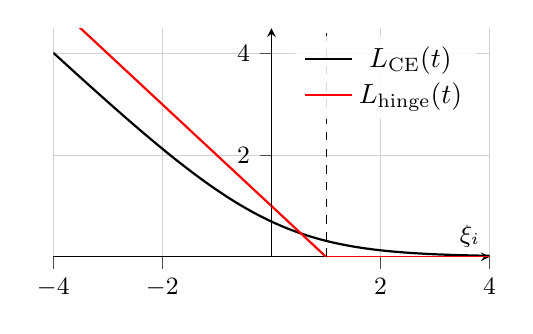
\begin{tikzpicture}
\begin{axis}[
  width=6.2cm, height=4cm,
  grid=both,
  grid style={line width=.1pt, draw=gray!20},
  major grid style={line width=.2pt, draw=gray!35},
  axis x line=middle,
  axis y line=middle,
  xlabel={$\xi_i$ },
  ylabel={},
  xmin=-4, xmax=4,
  ymin=0,  ymax=4.5,
  tick align=outside,
  tick style={black!70},
  label style={font=\small},
  tick label style={font=\small},
  legend pos=north east,
  legend style={draw=none, fill=white, fill opacity=0.85, text opacity=1},
  scale = 1.2
]
\addplot[domain=-4:4, samples=400, thick] {ln(1 + exp(-x))};
  \addlegendentry{$L_{\mathrm{CE}}(t)$}
  % --- Hinge: piecewise ---
  \addplot[domain=-4:1, samples=300, thick,red] {1 - x};
  \addplot[domain=1:4,  samples=2,   thick,red] {0};
  \addlegendentry{$L_{\mathrm{hinge}}(t)$}

  % --- Logistic (CE) ---
  

  % --- reference lines & points ---
  \addplot[very thin, dashed] coordinates {(1,0) (1,4.5)};
%   \node[anchor=west] at (axis cs:1,4.2) {$t=1$};

  \addplot[very thin, dashed] coordinates {(0,0) (0,4.5)};
%   \node[anchor=west] at (axis cs:0,3.2) {$t=0$};

  % L_ce(0) = ln 2
%   \addplot[only marks, mark=*] coordinates {(0,0.69314)};
%   \node[anchor=south east] at (axis cs:0,ln(2)) {$\ln 2$};

\end{axis}
\end{tikzpicture}
\end{document}